\documentclass[a4paper,12pt,titlepage]{report}
\usepackage[utf8]{inputenc}
\usepackage{graphicx}

\usepackage[footnotesize]{caption}

\makeatletter
\renewcommand{\fnum@figure}{\small\textbf{\figurename~\thefigure}}
\makeatother

\setcounter{secnumdepth}{-1} 

% Title Page
\title{Assignment Network Simulation}
\author{Peter De Wolf \& Wout Vekemans}
\begin{document}
\begin{titlepage}
	\maketitle
	\thispagestyle{empty}
\end{titlepage}

\section{Exercise 1: Bandwidth restrictions on Kotnet}
\begin{enumerate}
 \item When we leave out the uploading connection, the throughput of the FTP connection is relatively constant. See figure \ref{noUpload}. The throughput rate is limited by the bandwidth cap. 
  \begin{figure}[htb]
\centering
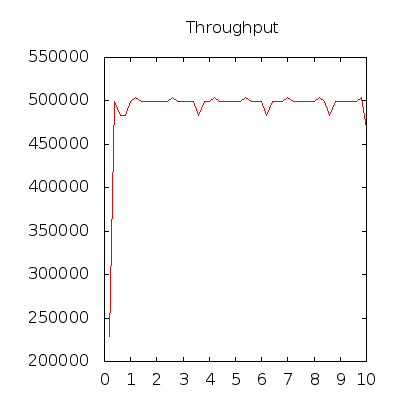
\includegraphics[width=0.5\textwidth]{noUpload.png}
\caption{Throughput of the main FTP connection}
\label{noUpload}
\end{figure}
% 2
\item When re-enabling the uploading connection, we see that the download rate drops when the upload starts. This is caused by the fact that the ACKs of the download need to travel through the same connection as the packets uploaded by the user. This results in a lot of dropped ACKs, which causes the server to restart sending, and therefore decreasing the throughput of the download link. See figure \ref{upAndDown}.\\
  \begin{figure}[htb]
\centering
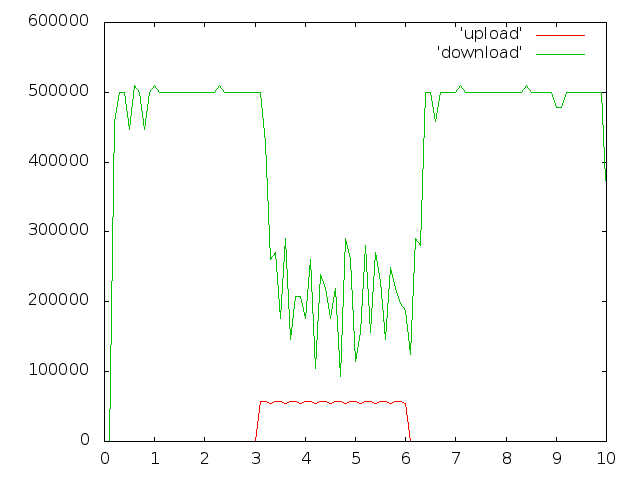
\includegraphics[width=0.5\textwidth]{withUpload.png}
\caption{Throughput of the FTP and UDP connection}
\label{upAndDown}
\end{figure}
% 3
\item When a fixed amount of upload bandwidth is allocated to both applications, there wont be a drop in the download throughput. It would be like there were to separate upload connections: one for the ACKs of the FTP connection, and one for the data packets of the CBR connection, so they would both have more or less constant throughput. The ACKs and the uploaded data packets would not 'steal' eachother's bandwidth. 
% 4
\item When the connection bandwidth is more limited, we get sort of the same result as in part 1, but with more packet loss. When the connection between server and user is slower, the buffers get full very fast, and more packets need to be dropped. This causes large fluctuations in download througput. \\
% 5
\item derp
% 6
\item 
\begin{enumerate}
  \item When there is 10 times more capacity and there are ten 10 equal users, the bandwidth will be equally divided between users. The only packet loss will be the ones 'accidentaly' getting lost, like in the first section of this question. //
  When there are five users wi
\end{enumerate}

\end{enumerate}


\section{Exercise 2: Tahoe and Reno versus bursty web traffic}
\begin{enumerate}
\item
In the beginning the buffers can compensate for the bursts. This causes for a delayed effect of the bursts. The bursts start to affect the connection once the buffers are completely filled. When this happens, the will be packet loss and the main FTP connection notices this loss. As response to this the main FTP connection will slow down the input rate (fast recovery to threshold followed by additive increase).

\item
The threshold in our example is 80. TCP uses slow start to converge to an optimal window size. In the beginning there will be an exponential increase of the congestion window until the threshold is reached. Once this occures, the congestion window will increase additive (AIMD). When the connection detects congestion, TCP uses fast recovery to avoid it. After the fast recovery decrease will occur until the size is half the size at which congestion was detected.

\item
AIMD or additive increase and multiple decrease is an algorithm used for TCP congestion avoidance. Additive increase and multiple decreases causes the size resemble a sawtooth wave.
This sawtooth converges around the optimum. Once the slow start threshold is reached, only additive increase is used by TCP to increase the congestion window. Fast recovery decreases the window size until it has half the size of the size at which congestion was detected. TCP does this using multiple decreases.

\item
The difference with the normal TCP is that Reno uses fast recovery. When one packet is lost, the congestion window decreases multiple times until the size is at half of the value of the window size at which congestion was detected. When more than one packet is lost, the window size decreases to zero.

\end{enumerate}

\end{document}          
